\textbf{\underline{OZ 6 - Magnetische inductie en de wet van Faraday - Oefening 5:}}
\vspace{0.5cm}

    Twee oneindig lange solenoïdes gaan door een circuit zoals aangegeven. De grootte van het magnetisch veld in beide solenoïdes is hetzelfde en neemt toe met $100$ T/s. Welke stromen lopen er door verschillende weerstanden?

    \begin{center}
        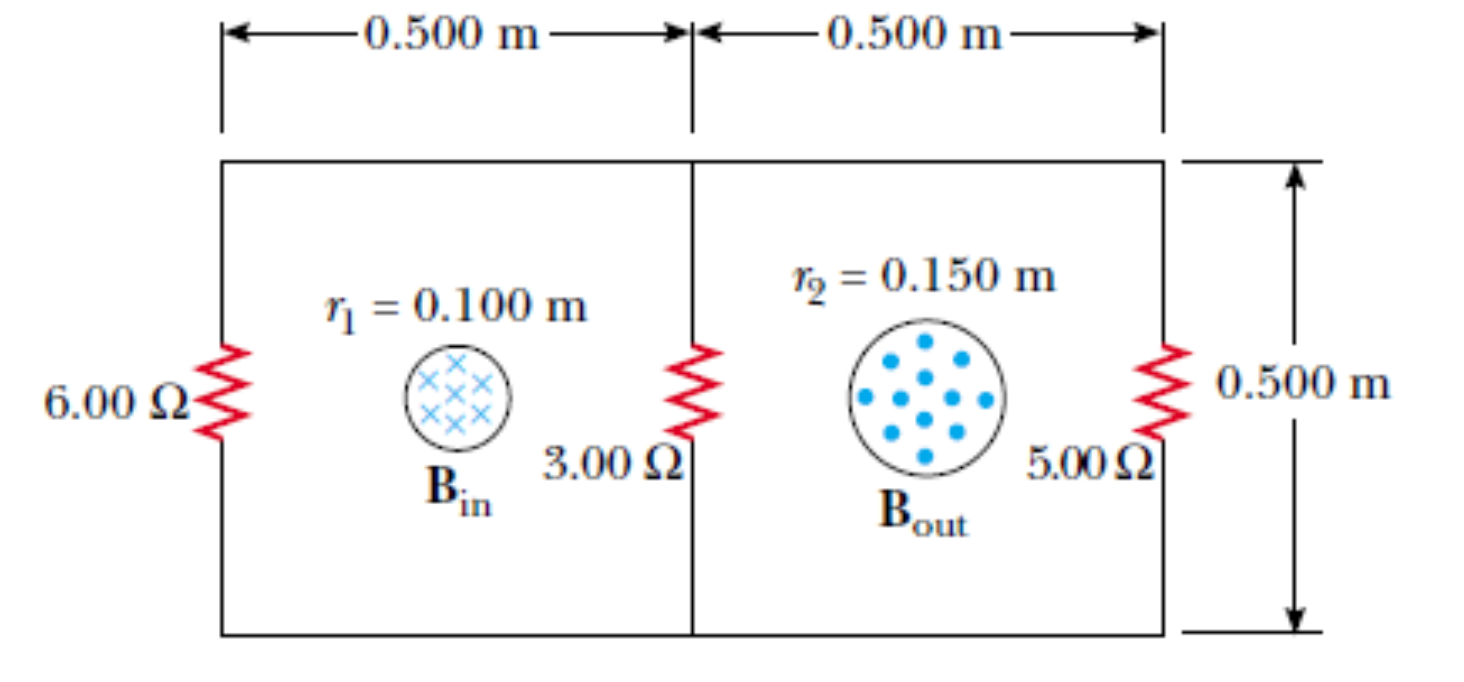
\includegraphics[scale = 0.3]{oz06/resources/Oz6Oef5.png}
    \end{center}

    \begin{description}[labelwidth=1.5cm, leftmargin=!]
        \item[Geg. :]
        \item[Gevr. :] 
        \item[Opl. :]
    \end{description}


\vspace{1cm}